\documentclass[]{scrartcl}
\usepackage[spanish]{babel}

\decimalpoint
%opening
\usepackage{xcolor}
\usepackage{mathtools}
\usepackage{graphicx}
\usepackage{enumitem}
\usepackage{hyperref}
\newcommand{\tt}[1]{\texttt{#1}}
\definecolor{bitacora}{HTML}{217821}
\newcommand{\that}[0]{\texttt{THAT~}}

\usepackage{siunitx}
\sisetup{output-decimal-marker = {.}}

\title{Práctica 1 de control: sistemas de primero y segundo orden mediante computación analógica \\}



\subtitle{\textcolor{bitacora}{\LARGE Incluya en su reporte solo lo que está en verde}}
\author{Leonardo Bermeo}

\begin{document}
	
	\maketitle


\section{Bloques de computación analógica básica}

El \tt{THAT} tiene varios bloques de computación analógica (multiplicadores, comparadores). Vamos a usar los siguientes bloques en esta práctica, junto con las convenciones mostradas en la figura~\ref{fig:tabla_analog}.
%
\begin{figure}[h!]
	\centering
	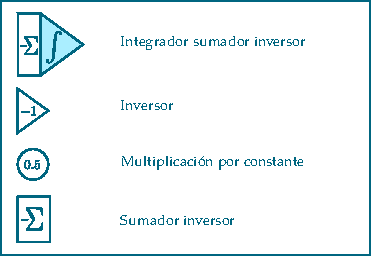
\includegraphics[width=0.6\linewidth]{figuras/tabla_analog}
	\caption{Bloques analógicos.}
	\label{fig:tabla_analog}
\end{figure}



\section{Sistema de Segundo orden}

Vamos a usar el \tt{THAT} para implementar sistemas de primero y segundo orden como los vistos en la teoría. Comenzaremos por un sistema de segundo orden con función de transferencia dada por:

\begin{equation}
	H(s)=\dfrac{Y(s)}{U(s)}=\dfrac{b_0}{s^2+a_1s + a_0}, \text{ con } b_0,a_1,a_0>0.
	\label{equ:Hs}
\end{equation}





Como sabemos, la representación en variables de estado de este sistema está dada por:
\begin{align*}
	\begin{bmatrix}
		\dot{x_1} \\
		\dot{x_2}
	\end{bmatrix}&=
	\begin{bmatrix}
		-a_1 & -a_0  \\
		1 & 0
	\end{bmatrix}	
	\begin{bmatrix}
		 x_1 \\
		 x_2
	\end{bmatrix} + 
		\begin{bmatrix}
		b_0 \\
		0
	\end{bmatrix} u 	\\
	y &= \begin{bmatrix}
		0 & 1
	\end{bmatrix}
		\begin{bmatrix}
		x_1 \\
		x_2
	\end{bmatrix}
\end{align*}
Es decir, las ecuaciones de estado para este sistema las podemos escribir como:
\begin{align}
	\dot{x}_1&= -a_1 x_1 -a_0  x_2 + b_0 u\nonumber\\
	\dot{x}_2&= x_1\nonumber\\
	y&=x_2\label{equ:est2orden}
\end{align}



\subsection{Implementación del sistema de segundo orden}
%
Con base en los bloques de computación analógica en la figura~\ref{fig:tabla_analog} vamos a implementar las ecuaciones de estado en \eqref{equ:est2orden}. Estas ecuaciones se implementan de acuerdo al  diagrama de computación analógica de la figura~\ref{fig:analog2order}:
 %
\begin{figure}[h!]
	\centering
	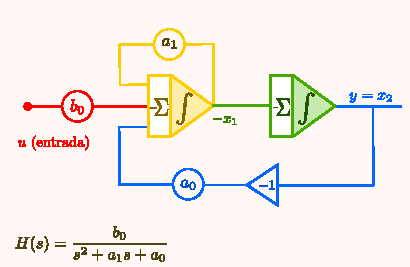
\includegraphics[width=0.6\linewidth]{figuras/seg_order_control}
	\caption{Implementación analógica del sistema de segundo orden.}
	\label{fig:analog2order}
\end{figure}
%
%Note que las variables de estado a la salida de los integradores siempre salen invertidas. Por ello, si suponemos que a la entrada del segundo integrador está $-x_1$ su salida debe ser $x_2$.
%
%\newpage
%
%\subsubsection{Pasos de Implementación en el THAT}
%\begin{enumerate}[label=\alph*)]
%	\item Identifique cada uno de los componentes del diagrama de la figura~\ref{fig:analog2orderthat}. Se puede guiar por la salidas de los integradores. Las lineas del diagrama de computación analógica están con los mismos colores sugeridos para las conexiones entre elementos del \tt{THAT}. Note que a la izquierda está la multiplicación por el coeficiente $b$ y a la derecha el inversor azul. 
% %
%\begin{figure}[h!]
%	\centering
%	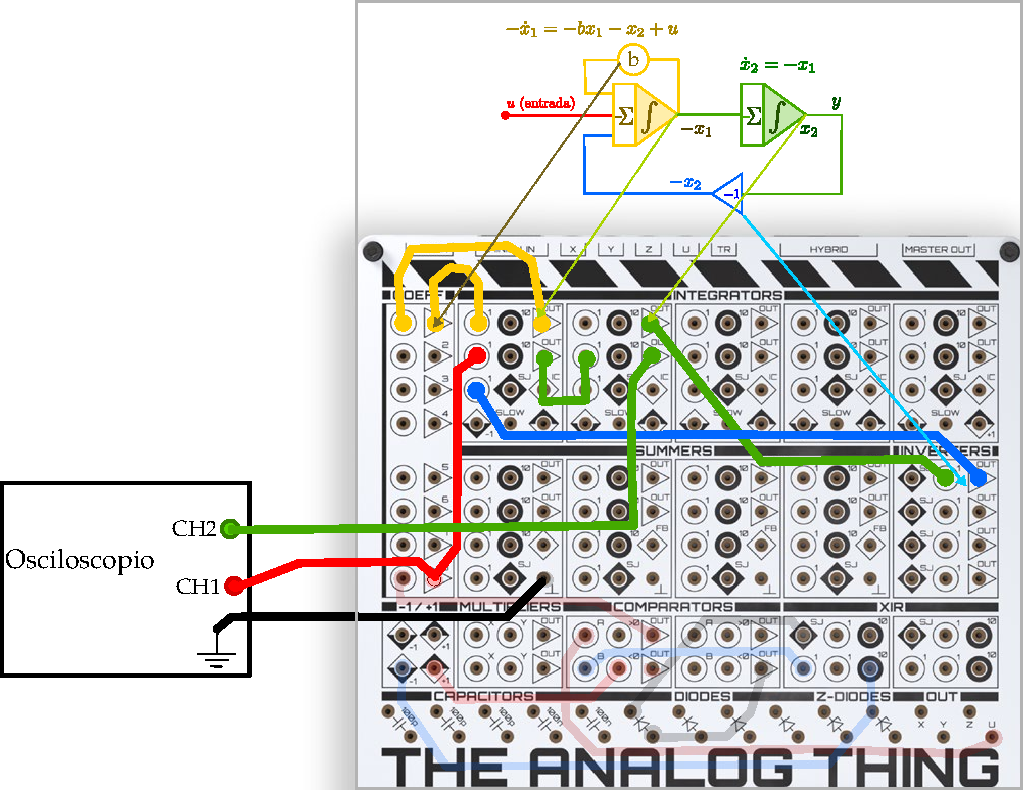
\includegraphics[width=0.9\linewidth]{figuras/analog2orderthat}
%	\caption{Implementación analógica del sistema de segundo orden.}
%	\label{fig:analog2orderthat}
%\end{figure}
%	\item Implementar cuidadosamente el diagrama de computador analógico de la figura~\ref{fig:analog2orderthat}. Note que no es necesario (ni deseable) conectar la tierra del canal 2.
%	\item Ponga la perilla \tt{MODE} del \tt{THAT} en \tt{COEFF} y ajuste el potenciómetro del coeficiente $b$ en 1. Regrese la perilla al modo \tt{REPF}.
%	
%	\newpage
%	\item Sincronice los dos canales del osciloscopio para ver la respuesta al escalón del sistema de segundo orden implementado. Use como fuente de sincronia el escalón (canal 1) y ajuste el trigger apropiadamente para obtener una imagen fija. Debe estar obteniendo una respuesta similar a esta:
%	%
%	\begin{figure}[h!]
%		\centering
%		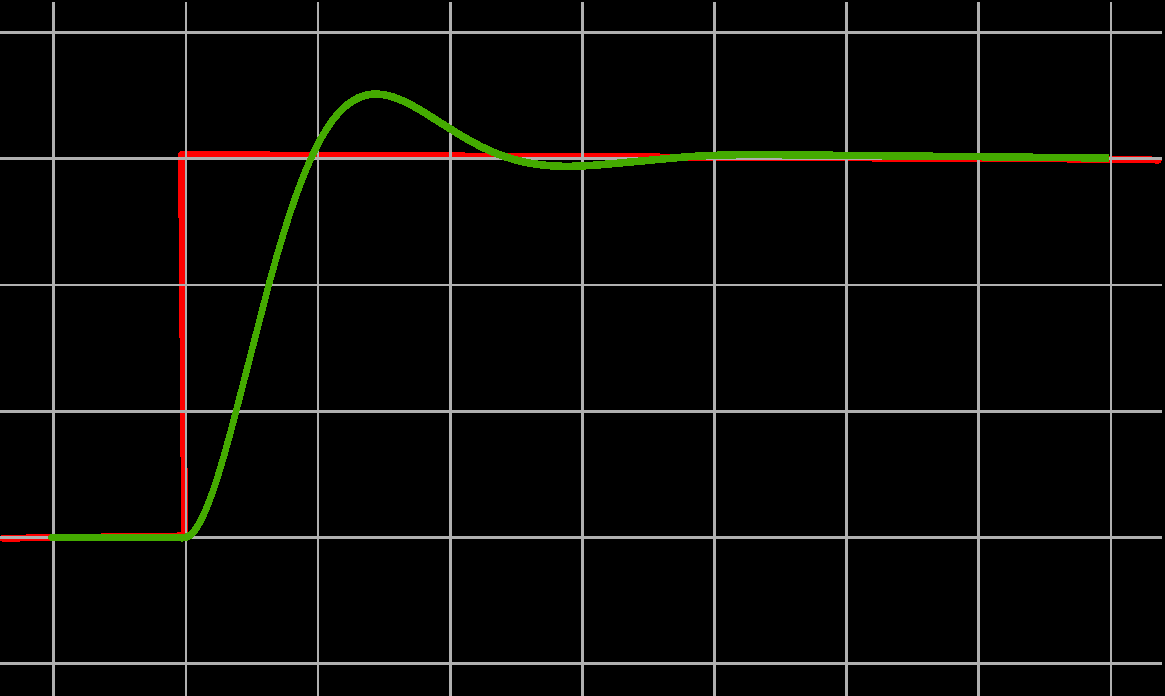
\includegraphics[width=0.6\linewidth]{figuras/osc}
%		\caption{Señal del sistema de segundo orden}
%		\label{fig:senal2orden}
%	\end{figure}
%	\item Varie suavemente el valor del potenciométro de  $b$ y observe lo que ocurre. Discuta con su compañero.
%	\item Obtenga la respuesta para valores de $b$ = 0, 0.25, 0.5, 1. No es necesario ser tan preciso. Haga con su compañero un bosquejo aproximado de la localización de los polos en el plano complejo para estos valores de $b$. Indique si hay casos en que el sistema es inestable.
%
%	\item Acceda a \href{https://colab.research.google.com/drive/1b7orSCMo12l76fKedXTSs88f4nAhV3Ly?usp=sharing}{este notebook de colab}, ejecute cada una de las celdas, compare con su bosquejo y los resultados que obtuvo.
%	\item ¿Qué valor mínimo de $b$ necesitamos para obtener un sistema amortiguado (sin oscilaciones, con polos reales)? 
%	\item ¿Cómo podemos obtenerlo en el \tt{THAT}? Revise la sección~\ref{sec:coefmay} y produzca un sistema amortiguado, sin oscilaciones. 
%	
%\end{enumerate}
%
%\subsubsection{Sistema inestable}
%
%Ahora vamos a implementar el mismo sistema de segundo orden pero con un pequeño cambio. La función de transferencia que vamos a implementar  es ahora la siguiente:
%\begin{equation}
%	H(s)=\dfrac{1}{s^2-bs+1}, b>0.	
%	\label{equ:inestable}
%\end{equation}
%
%Note para implementar la ecuación~\eqref{equ:inestable} solo es necesario colocar un inversor para $b$ como se ilustra a continuación:
% %
%\begin{figure}[h!]
%	\centering
%	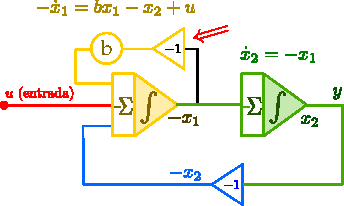
\includegraphics[width=0.5\linewidth]{figuras/analog2orderinest}
%	\caption{Implementación analógica del sistema de segundo orden con coeficiente  negativo.}
%	\label{fig:2orderinestable}
%\end{figure}
%
%\begin{enumerate}[label=\alph*)]
%	\item Discuta con su compañero de trabajo si el sistema de la ecuación~\eqref{equ:inestable} es estable o inestable.
%
%	\item Realice esta modificación en el  \tt{THAT} para implementar el sistema de la figura~\ref{fig:2orderinestable}.
%	 %
%	\begin{figure}[h!]
%		\centering
%		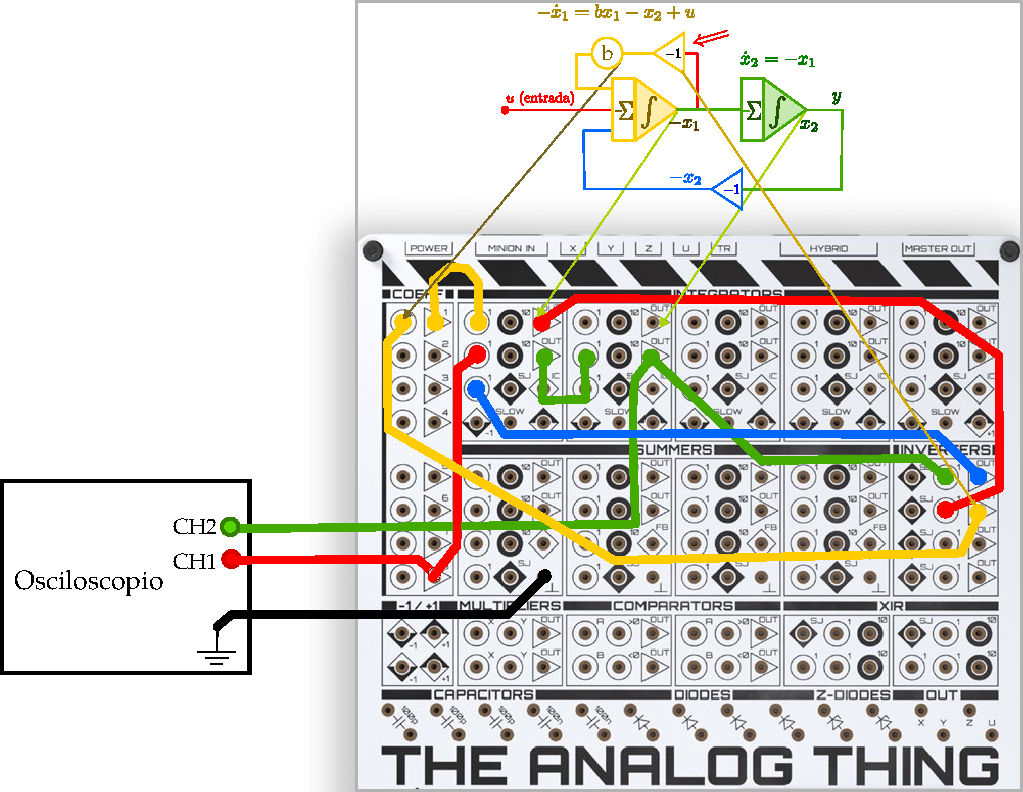
\includegraphics[width=0.9\linewidth]{figuras/analog2orderthatinest}
%		\caption{Implementación analógica del sistema de segundo orden con coeficiente negativo.}
%		\label{fig:analog2orderinest}
%\end{figure}
%
%\item Ajuste la tensión del escalón de entrada con \tt{COEFF 8} en aproximadamente 1V. Sincronice el osciloscopio con este escalón.
%\item Varie suavemente el valor de $b$ y observe lo que ocurre.
%\item Discuta lo que ocurre cuando $b=.05$ y cuando $b=0.1$. Haga un bosquejo de la ubicación de los polos del sistema en el plano complejo para estos casos.
%\item Discuta sobre la estabilidad de este sistema.
%\item Compare sus resultados con los que se obtienen en \href{https://colab.research.google.com/drive/1yLNEhGWMdqoO_5xwOrW4sqK69zA014Ml?usp=sharing}{este colab}
%\end{enumerate}

%\section{Sistema de lazo cerrado y test de Rooth-Hurwitz}
%\newpage
%\section{Filtro analógico de Chebyschev}
%
%\subsection{Especificaciones y diseño}
%
%En esta parte vamos a implementar un filtro analógico con las siguientes especificaciones:
%
%\begin{itemize}
%	\item Frecuencia de corte real: $f_{p,real}=100\,\text{Hz}$
%	\item Rizado en la banda de paso: $\alpha_P=0.1\,\text{dB}$
%	\item Atenuación en la banda de rechazo: $\alpha_S=25\text{dB}$
%\end{itemize}
%
%\emph{Nota:} Los condensadores y resistencias del \tt{THAT} no se pueden cambiar. Como el \tt{THAT} tiene resistencias y condensadores en los  integradores con constante de tiempo $RC=1M\Omega \times 1\text{nF} = 0.001s$, asumiremos que la frecuencia angular normalizada  para el \tt{THAT} es de
%
%\[ 1/RC=1/0.01=1000\text{rad/s.}\]
%
%Esto quiere decir que con los coeficientes numéricos que obtendremos para un filtro con frecuencia normalizada en 1, la frecuencia de corte del \tt{THAT} será $\overline{\omega_P}=1000\text{rad/s}$, esto es, $159.15\text{Hz}$. 
%
%Si requerimos un filtro para una frecuencia de $100Hz$, debemos diseñar para la frecuencia
%
%\[\omega_p= \dfrac{2\times \pi \times f_{p,real}}{1000}=  \dfrac{2\times \pi \times 1000}{100}=0.628\, \text{rad/s}\] 
%
%
%En este \href{https://colab.research.google.com/drive/1FAwNfmSHj2Xydje-8FpgHDbYV_laZE4f?usp=sharing}{notebook de colab} está el diseño del filtro para la frecuencia  $f_{p,real}=100\,\text{Hz}$ requerida.
%
%
%\subsection{Implementación del filtro analógico}
%
%Una vez diseñado el filtro obtenemos una función de transferencia en secciones de segundo orden dada por:
%\begin{equation}
%	H(s)= \underbrace{\dfrac{0.128}{s^2 + 0.801\,s + 0.246}}_{H_1(s)} \times \underbrace{\dfrac{1}{s^2 + 0.332\,s + 0.525}}_{H_2(s)} 
%	\label{equ:filcheb}          
%\end{equation} 
%Vamos a escribir el filtro de la ecuación~\eqref{equ:filcheb} de la siguiente forma más general: 
%\begin{equation}
%	H(s)= \underbrace{\dfrac{b_{0}}{s^2 + a_{11}\,s + a_{01}}}_{H_1(s)} \times \underbrace{\dfrac{1}{s^2 + a_{12}\,s + a_{02}}}_{H_2(s)}
%	\label{equ:filchebgen}          
%\end{equation} 
%
%La implementación de la función de transferencia $H(s)=H_1(s)\times H_2(s)$ de la ecuación~\eqref{equ:filchebgen} se puede realizar de acuerdo al diagrama de computación analógica mostrado en la figura~\ref{fig:filtrocomp}.
%	 %
%\begin{figure}[th!]
%	\centering
%	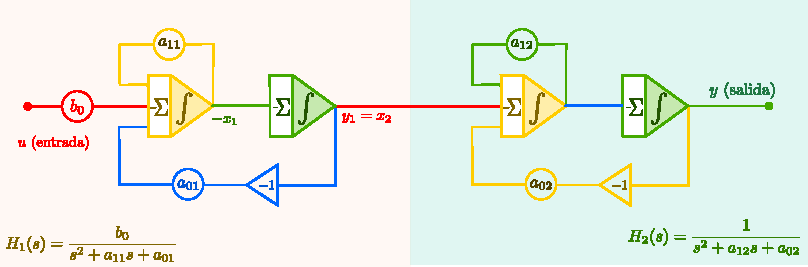
\includegraphics[width=1\textwidth]{figuras/filtrocomp}
%	\caption{Diagrama de computación analógica del filtro de la ecuación \eqref{equ:filchebgen}.}
%	\label{fig:filtrocomp}
%\end{figure}
%
%Para mostrar que esa es implementación analógica consideremos las ecuaciones de estado de $H_1(s)$, dadas por: 
%
%\begin{align}
%	\dot{x_1}&= -a_{11}\,x_1 - a_{01} x_2 + b_0\,u\nonumber\\
%	\dot{x_2}&= x_1\nonumber\\
%	y_1&=x_2
%\end{align}
%Note que justamente el diagrama de computación analógica de la izquierda corresponde con esta descripción de estado (teniendo en cuenta que los integradores son inversores). De forma similar construimos $H_2(s)$.
%
%
\newpage
\subsection{Pasos de implementación en el \tt{THAT}}

\begin{enumerate}[label=\alph*)]
%\item ``Resetee el \that'', es decir, retire todos los conectores, incluido el RCA. Ponga el \that en modo  \tt{OFF}.

%\newpage
\item  Conecte el generador de ondas a la entrada \tt{Z} como se muestra en la figura~\ref{fig:generador}, usando el adaptador BNC-RCA provisto.
 %
\begin{figure}[h!]
	\centering
	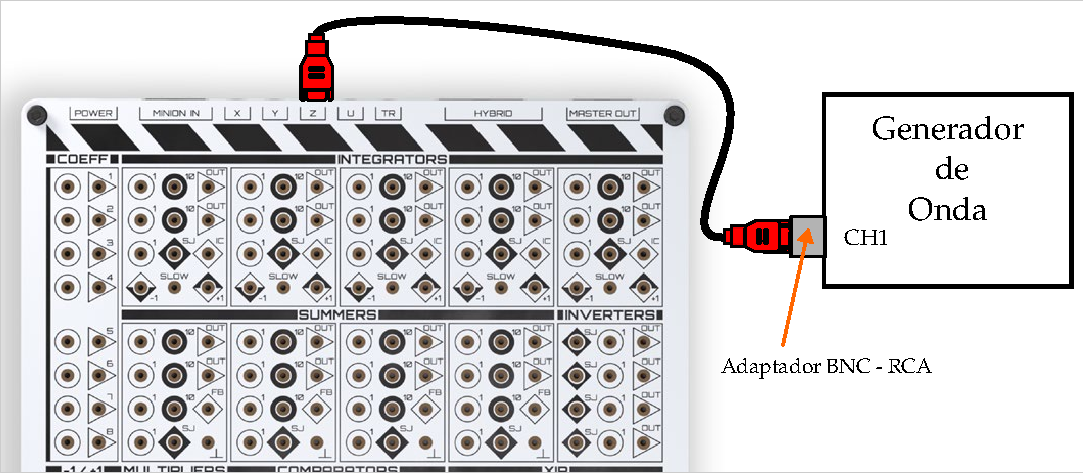
\includegraphics[width=0.7\textwidth]{figuras/generador}
	\caption{Conexión del generador de ondas.}
	\label{fig:generador}
\end{figure}
\item Identifique claramente cada uno de los componentes del diagrama de la figura~\ref{fig:seg_orden_real} que implementa la función de transferencia $H(s)$ de la ecuación~\eqref{equ:Hs}.
%
\begin{figure}[h!]
	\centering
	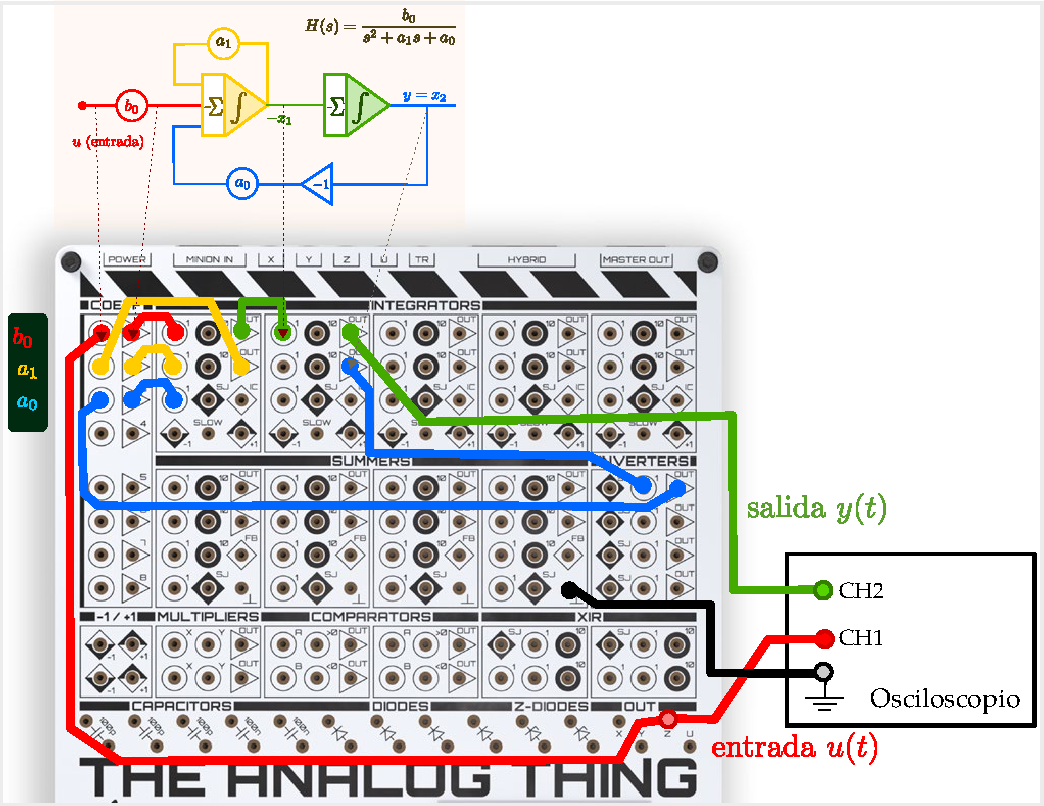
\includegraphics[width=0.9\textwidth]{figuras/seg_order_that.pdf}
	\caption{Implementación del filtro en el \that.}
	\label{fig:seg_orden_real}
\end{figure}

Note que los coeficientes de las funciones de transferencia están asociados con los controles \tt{COEFF} del \that que están en los potenciómetros abajo,  como se ilustra en la figura~\ref{fig:potenciometros}.
%
\begin{figure}[h!]
	\centering
	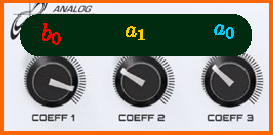
\includegraphics[width=0.5\textwidth]{figuras/potenciometros.pdf}
	\caption{Implementación del filtro en el \that.}
	\label{fig:potenciometros}
\end{figure}

\item  Implementar cuidadosamente el diagrama de computador analógico de la figura~\ref{fig:seg_orden_real}. Note que no es necesario (ni deseable) conectar la tierra del canal 2.

\item Ajuste el generador de onda con una señal cuadrada de $10\,\text{Hz}$. Ajuste la tensión del generador en  $4V_{pp}$. Ajuste el offset en $2\,V$ para que la señal inicie en cero y sincronice apropiadamente el osciloscopio con \textbf{\textcolor{red}{con el acoplamiento de ambos canales en DC!}} Debe obtener una señal como la mostrada en la figura \ref{fig:ondacuadrada}
%
\begin{figure}[h!]
	\centering
	
\includegraphics[width=0.5\textwidth]{figuras/onda_cuadrada.pdf}
	\caption{Entrada al sistema de segundo orden \that.}
	\label{fig:ondacuadrada}
\end{figure}

\subsection{Trabajo experimental del laboratorio}
 
Vamos a implementar un sistema de segundo orden de la forma:

\begin{equation}
H(s)=\dfrac{\omega_n^2}{s^2 + 2 \zeta \omega_n s + \omega_n^2}
\label{equ:Hslab},
\end{equation}
usando la realización de estado de  la ecuación~\eqref{equ:est2orden}, implementada en el \that en la figura~\eqref{fig:seg_orden_real}. 

\subsubsection*{Pasos}

\begin{enumerate}
	\item \textcolor{bitacora}{Encuentre los coeficientes $b_0$, $a_1$ y $a_0$ para obtener un $\omega_n=0.5$ y un $\zeta =0.5$}
	  
	\item Ponga el \that en modo \tt{COEFF} y ajuste cuidadosamente cada uno de los coeficientes del sistema. Por ejemplo, para ajustar el coeficiente $b_0$ ponga la perilla \tt{COEFFICIENT} en \tt{1} y ajuste el potenciómetro rotulado como \tt{COEFF1}, como se muestra en la figura~\ref{fig:coeffs}. El display mostrará el valor actual de $b_0$.
	%
	\begin{figure}[h!]
		\centering
		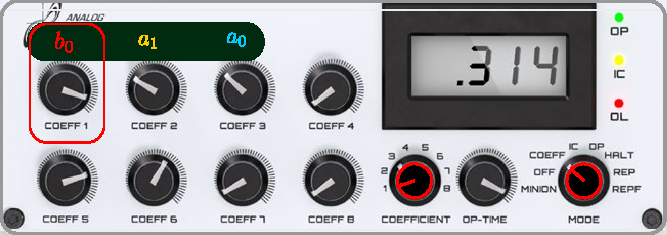
\includegraphics[width=0.7\textwidth]{figuras/coeffs.pdf}
		\caption{Ajuste de coeficientes de la función de transferencia en el  \that.}
		\label{fig:coeffs}
	\end{figure}
	
	
  	\item  Ponga el \tt{THAT} en el modo \tt{OP} (modo de operación sin reset). Sincronice los dos canales del osciloscopio para ver la respuesta al escalón del sistema de segundo orden implementado. Use como fuente de sincronía el escalón (canal 1) y ajuste el trigger apropiadamente para obtener una imagen fija. Debe estar obteniendo una respuesta similar a la de la figura \ref{fig:senal2orden}.
  	%
  	\begin{figure}[h!]
  			\centering
  			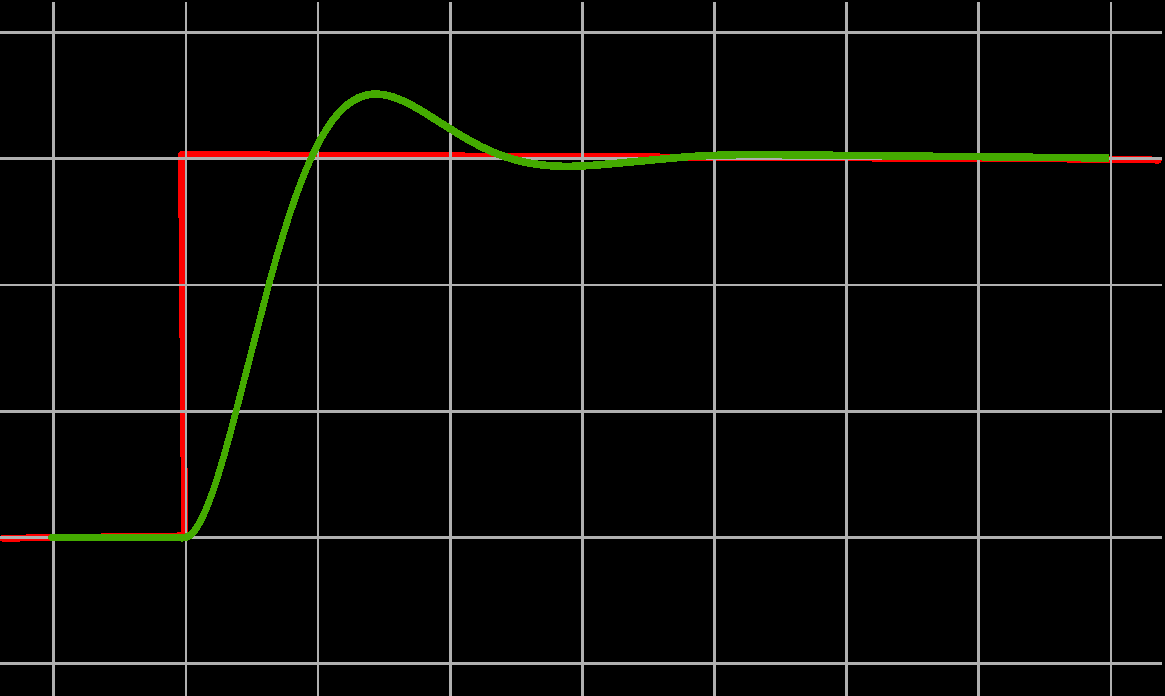
\includegraphics[width=0.6\linewidth]{figuras/osc}
  			\caption{Señal del sistema de segundo orden}
  			\label{fig:senal2orden}
  		\end{figure}

	
%	\item \textcolor{bitacora}{Encuentre experimental y analíticamente la respuesta de estado estacionario $y_{ee}(t)$ del sistema ante el escalón aplicado.}
	
	\item \textcolor{bitacora}{Calcule el valor de $\zeta$ que necesita para obtener un sobrepico de $5$, $10\%$, y $40\%$. Prográmelo en el THAT  yregistre  el sobrepico real obtenido, el tiempo de subida y el tiempo de establecimiento (aproximado, claro está). Haga una tabla con los valores obtenidos y los que se obtienen de las expresiones matemáticas para estos casos.}  \\
	

	
	\textcolor{red}{\emph{Note que el THAT tiene una escala de tiempo (1:1000), es decir cada milisegundo del THAT es 1 segundo del sistema que estamos implementando.}}
\end{enumerate}

\section{Sistema de primer orden} 

Ahora vamos a usar el THAT para implementar un sistema de primer orden de la forma: 
\begin{equation}
 G(s)=\dfrac{b}{s+a}.
 \label{equ:primorden}
 \end{equation}
 
\subsubsection*{Pasos}

\begin{enumerate}
	
	\item  \textcolor{bitacora}{Encuentre los parámetros $b$ y $a$ de la ecuación~\ref{equ:primorden} para satisfacer los siguientes requerimientos de diseño:}
	\begin{itemize}
		\item Tiempo de subida cercano a 11.5 segundos.
		\item Respuesta en estado estacionario a un escalón que sea del doble de la amplitud del escalón.
	\end{itemize}
	
	\item \textcolor{bitacora}{diseñe un diagrama de computación analógica (el dibujo) que implemente la función anterior.}
	
	\item Implemente en el THAT el diseño de computación analógica.
	
	\item  \textcolor{bitacora}{Registre el tiempo de subida y la respuesta de estado estacionario y compare con los valores de los requerimientos de diseño. Incluya los gráficos del osciloscopio.}
	

\end{enumerate} 
\end{enumerate}

\textcolor{red}{\Large Al finalizar incluyan reflexiones propias sobre esta práctica que no sean generadas con IA. Prefiero que se resignen y escriban: ``no se nos ocurrió nada'', antes de generar artefactos de texto que les impiden  cerrar el circuito de aprendizaje.}

\end{document}
